\documentclass[11pt,spanish,a4paper]{article}
% Versión 2.o cuat 2014 Víctor Bettachini < bettachini@df.uba.ar >

\usepackage{babel}
\addto\shorthandsspanish{\spanishdeactivate{~<>}}
\usepackage[utf8]{inputenc}
\usepackage{float}

\usepackage{units}
\usepackage[separate-uncertainty=true, multi-part-units=single, locale=FR]{siunitx}

\usepackage{amsmath}
\usepackage{amstext}
\usepackage{amssymb}

% \usepackage{enumerate}

\newcommand{\pvec}[1]{\vec{#1}\mkern2mu\vphantom{#1}}

\usepackage{tikz}
\usepackage{xparse}
\usetikzlibrary{calc}

\tikzset{%
    Cote node/.style={%
        midway,
        sloped,
        fill=white,
        inner sep=1.5pt,
        outer sep=2pt
    },
    Cote arrow/.style={%
        <->,
        >=latex,
        very thin
    }
}

\makeatletter
\NewDocumentCommand{\Cote}{%
    s       % cotation avec les flèches à l'extérieur
    D<>{1.5pt} % offset des traits
    O{.75cm}    % offset de cotation
    m       % premier point
    m       % second point
    m       % étiquette
    D<>{o}  % () coordonnées -> angle
            % h -> horizontal,
            % v -> vertical
            % o or what ever -> oblique
    O{}     % parametre du tikzset
    }{%

    {\tikzset{#8}

    \coordinate (@1) at #4 ;
    \coordinate (@2) at #5 ;

    \if #7v % Cotation verticale
        \coordinate (@0) at ($($#4!.5!#5$) + (#3,0)$) ; 
        \coordinate (@4) at (@0|-@1) ;
        \coordinate (@5) at (@0|-@2) ;
    \else
    \if #7h % Cotation horizontale
        \coordinate (@0) at ($($#4!.5!#5$) + (0,#3)$) ; 
        \coordinate (@4) at (@0-|@1) ;
        \coordinate (@5) at (@0-|@2) ;
    \else % cotation encoche
    \ifnum\pdfstrcmp{\unexpanded\expandafter{\@car#7\@nil}}{(}=\z@
        \coordinate (@5) at ($#7!#3!#5$) ;
        \coordinate (@4) at ($#7!#3!#4$) ;
    \else % cotation oblique    
        \coordinate (@5) at ($#5!#3!90:#4$) ;
        \coordinate (@4) at ($#4!#3!-90:#5$) ;
    \fi\fi\fi

    \draw[very thin,shorten >= #2,shorten <= -2*#2] (@4) -- #4 ;
    \draw[very thin,shorten >= #2,shorten <= -2*#2] (@5) -- #5 ;

    \IfBooleanTF #1 {% avec étoile
    \draw[Cote arrow,-] (@4) -- (@5)
        node[Cote node] {#6\strut};
    \draw[Cote arrow,<-] (@4) -- ($(@4)!-6pt!(@5)$) ;   
    \draw[Cote arrow,<-] (@5) -- ($(@5)!-6pt!(@4)$) ;   
    }{% sans étoile
    \ifnum\pdfstrcmp{\unexpanded\expandafter{\@car#7\@nil}}{(}=\z@
        \draw[Cote arrow] (@5) to[bend right]
            node[Cote node] {#6\strut} (@4) ;
    \else
    \draw[Cote arrow] (@4) -- (@5)
        node[Cote node] {#6\strut};
    \fi
    }}
    }
\makeatother

\usetikzlibrary{decorations.pathmorphing, patterns}

\usepackage{graphicx}
\graphicspath{{./graphs_descripcion/}}

\voffset-3.5cm
\hoffset-3cm
\setlength{\textwidth}{17.5cm}
\setlength{\textheight}{27cm}

\usepackage{lastpage}
\usepackage{fancyhdr}
\pagestyle{fancyplain}
\fancyhead{}
% \fancyhead{{\tiny Física 2(F) - Prof. Skigin - 2"o cuat. 2014}}
\fancyfoot{{\tiny \textcopyright Departamento de Física, FCEyN, UBA}}
\fancyfoot[C]{ {\tiny Actualizado al \today} }
\fancyfoot[RO, LE]{Pág. \thepage/\pageref{LastPage}}
\renewcommand{\headrulewidth}{0pt}
\renewcommand{\footrulewidth}{0pt}


\begin{document}
\begin{center}
  \textbf{Física 2} (Físicos) \hfill \textcopyright {\tt DF, FCEyN, UBA}\\
  \textsc{\LARGE Descripción geométrica de movimientos ondulatorios}
\par\end{center}{\large \par}



\begin{enumerate}

\section*{Fermat, Snell}


\item 
\begin{enumerate}
	\item Si un rayo parte del punto $A=(0,1,0)$, se refleja en el espejo plano
$(x,0,z)$ y pasa por el punto $B=(4,3,0)$, averigüe en qué punto
sobre el plano del espejo se refleja y los ángulos de incidencia y
reflexión. Aplicar Fermat e interpretar físicamente las soluciones. 
	\item Un rayo directo entre $A$ y $B$ recorre un menor camino óptico que
el hallado en (a), ¿es esto contradictorio?
\end{enumerate}


\item A partir del principio de Fermat deducir la ley de Snell para la refracción
de la luz entre dos medios de índices $n_{1}$ y $n_{2}$, separados
por una superficie plana.
i

\item Sea un espejo elíptico de focos $A$ y $B$. En $A$ hay una fuente
puntual. Los espejos esférico y plano dibujados son tangentes al elíptico
en $C$. Sabiendo que el camino óptico de un rayo que sale de $A$,
se refleja en $C$ y luego pasa por $B$, es estacionario en la elipse,
obtenga cualitativamente si el camino óptico es máximo, mínimo o estacionario
cuando se refleja en cada uno de los espejos.


\section*{Prisma}
\item  
\begin{enumerate}
\item Demuestre que un rayo que incide sobre una lámina de caras paralelas,
inmersa en un medio único, no se desvía al atravesarla. Calcule el
desplazamiento lateral de dicho rayo, en términos de su espesor $d$
y de su índice de refracción $n$.
\item Demuestre que el rayo que se refleja en la primera cara y el que emerge
luego de reflejarse en la segunda son paralelos.
\item Si el medio exterior es único, ¿existe algún ángulo de incidencia
tal que produzca reflexión total en la cara inferior?
\end{enumerate}
\item Un rayo incide con ángulo $\phi$ sobre la superficie horizontal de
un cubo de material transparente, de índice $n$, inmerso en aire.
\begin{figure}[H]
\centering{}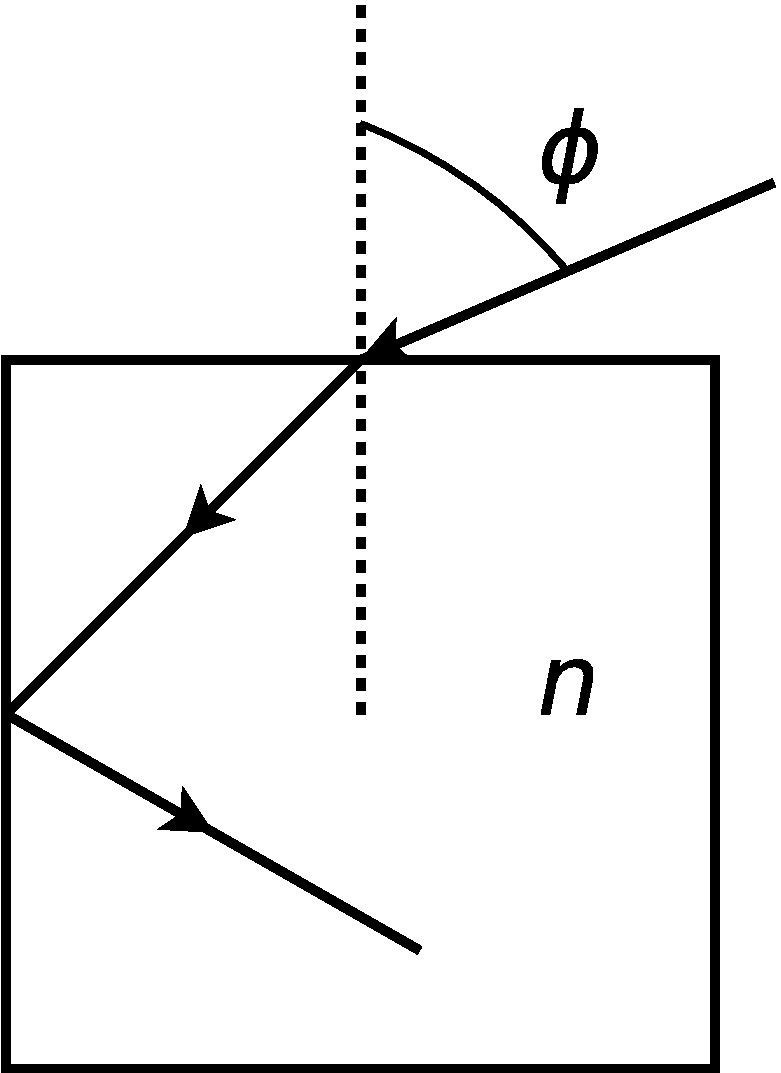
\includegraphics[clip,scale=0.25]{ej3-5}
\end{figure}


\begin{enumerate}
\item ¿Para qué valores de $\phi$ hay reflexión total en la cara vertical?
\item Si $\phi=60^{\circ}$, ¿cuál es el máximo $n$ para que no haya reflexión
total en la cara vertical? ¿Se puede reflejar totalmente en la cara
superior?
\end{enumerate}


%\item ~

\begin{enumerate}
\item Calcule analíticamente el ángulo de desviación mínima del prisma.
Justifique por qué este valor es único. Haga un gráfico cualitativo
de la desviación como función del ángulo de incidencia.
\item Calcule la desviación mínima para prismas delgados, en función de
los datos constructivos.
\item Si el prisma es delgado y el ángulo de incidencia es pequeño, calcule
la desviación.
\end{enumerate}


\item Los índices de refracción de cierta clase de vidrio para el rojo y
el violeta valen: $1.51$ y $1.53$; respectivamente. Halle los ángulos
límites de reflexión total para rayos que incidan en la superficie
de separación vidrio-aire. ¿Qué ocurre si un rayo de luz blanca incide
formando un ángulo de 41$^{\circ}$ sobre dicha superficie?


\section*{Espejo plano}


\item
\begin{enumerate}
\item En un vidrio óptico común se propaga un haz de luz blanca, ¿qué componente
viaja más rápido: la roja o la violeta?
\item ¿Para cuál de ambos colores será mayor la desviación en un prisma?
¿Qué puede decir del ángulo de desviación mínima? Justifique sus respuestas.
\end{enumerate}


\item Dado un prisma de Crown de ángulo $\alpha=4^{\circ}$ calcular, para
las líneas F, D y C, las desviaciones de rayos que inciden casi perpendicularmente.
Los respectivos índices son: $n_{F}=1.513$; $n_{D}=1.508$ y $n_{C}=1.504$.


\item 
\begin{enumerate}
\item Demuestre que la imagen dada por un espejo plano de una fuente puntual
es, sin ninguna aproximación, otra fuente puntual, ubicada simétricamente
respecto del plano del espejo. Analice los casos que corresponden
a objetos reales o virtuales.
\item ¿Cuál es la mínima longitud de un espejo plano vertical para que un
hombre de $1.8$ m se vea entero? ¿Es importante conocer la distancia
hombre-espejo? 
\end{enumerate}


\item Haga un esquema de un diagrama de rayos localizando las imágenes de
la flecha que se muestra en la figura. Para un punto de la flecha
dibuje una porción del frente de ondas emergente y los correspondientes
frentes reflejados.
\begin{figure}[H]
\centering{}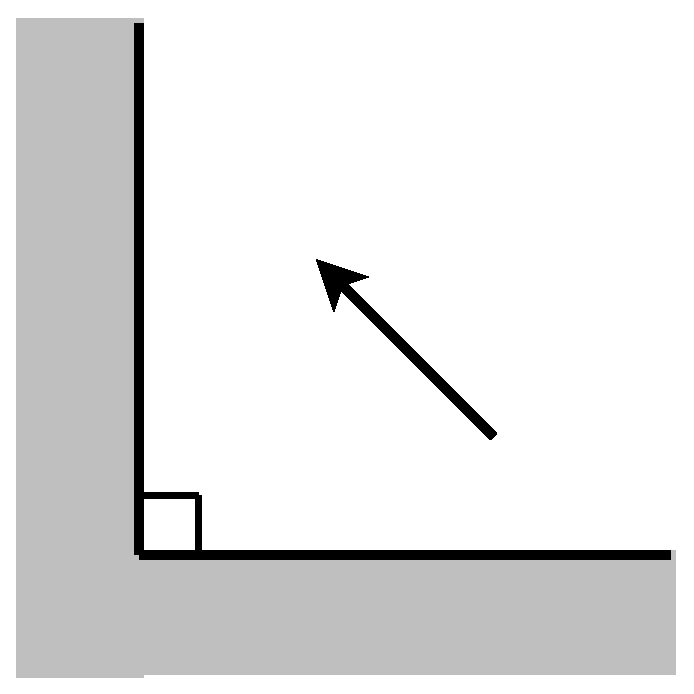
\includegraphics[clip,scale=0.25]{ej3-11}
\end{figure}



\item Dos espejos planos forman un ángulo $\alpha$ como lo indica la figura.
\begin{figure}[H]
\centering{}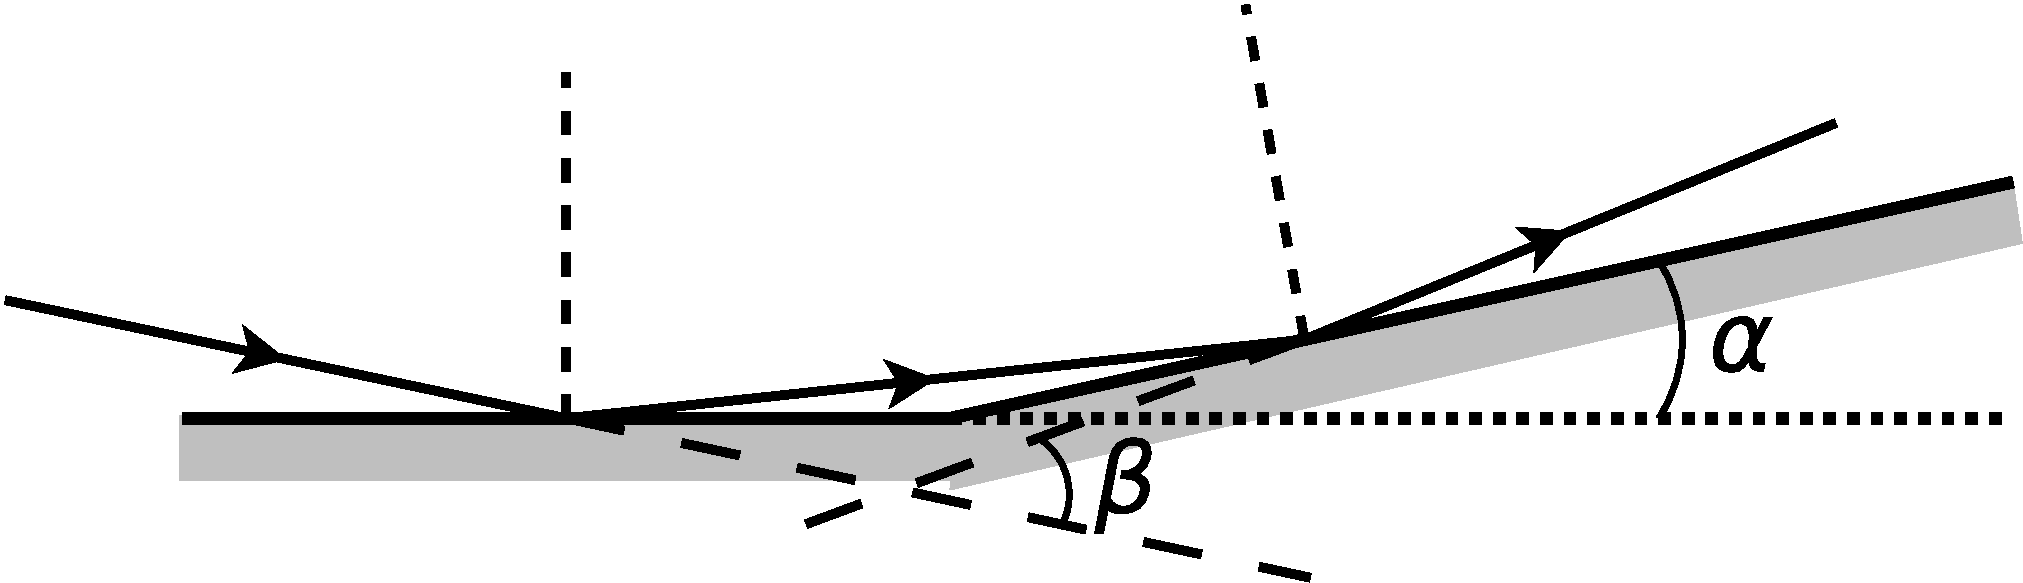
\includegraphics[clip,scale=0.25]{ej3-12}
\end{figure}


\begin{enumerate}
\item Un rayo de luz contenido en un plano perpendicular a la intersección
de los espejos incide sobre uno de ellos, se refleja e incide en el
otro (ver figura). Calcule el ángulo que forman los rayos incidente
y emergente.
\item Suponga la misma geometría que en (a) pero ahora iluminada por una
fuente puntual, demuestre que las imágenes se encuentran sobre una
circunferencia con centro en el vértice de los espejos. En el caso
en que la fuente está ubicada de tal modo que sólo se producen dos
imágenes, y que el ángulo es muy pequeño, calcule la distancia entre
ellas (espejos de Fresnel).
\end{enumerate}


\section*{Dioptra}

\item 
\begin{enumerate}
\item Demostrar que un haz homocéntrico de pequeña abertura que incide casi
normal sobre una dioptra plana, da lugar a otro haz homocéntrico.
Considere los casos de objetos reales y virtuales.
\item Una moneda se encuentra en el fondo de un vaso que contiene agua hasta
una altura de 5 cm ($n_{agua}=1.33$). Un observador la mira desde
arriba, ¿a qué profundidad la ve?
\item Estimar la máxima abertura de un haz homocéntrico, para que la posición
de la imagen, formada por una única superficie plana, quede determinada
con un error del 2\%. 
\end{enumerate}
\item Usando los resultados del problema anterior demuestre que un haz homocéntrico
de pequeña abertura, al atravesar una lámina de caras paralelas, da
lugar, en primera aproximación, a otro haz homocéntrico. Halle la
posición de las sucesivas imágenes. 


\item
\begin{figure}[H]
\centering{}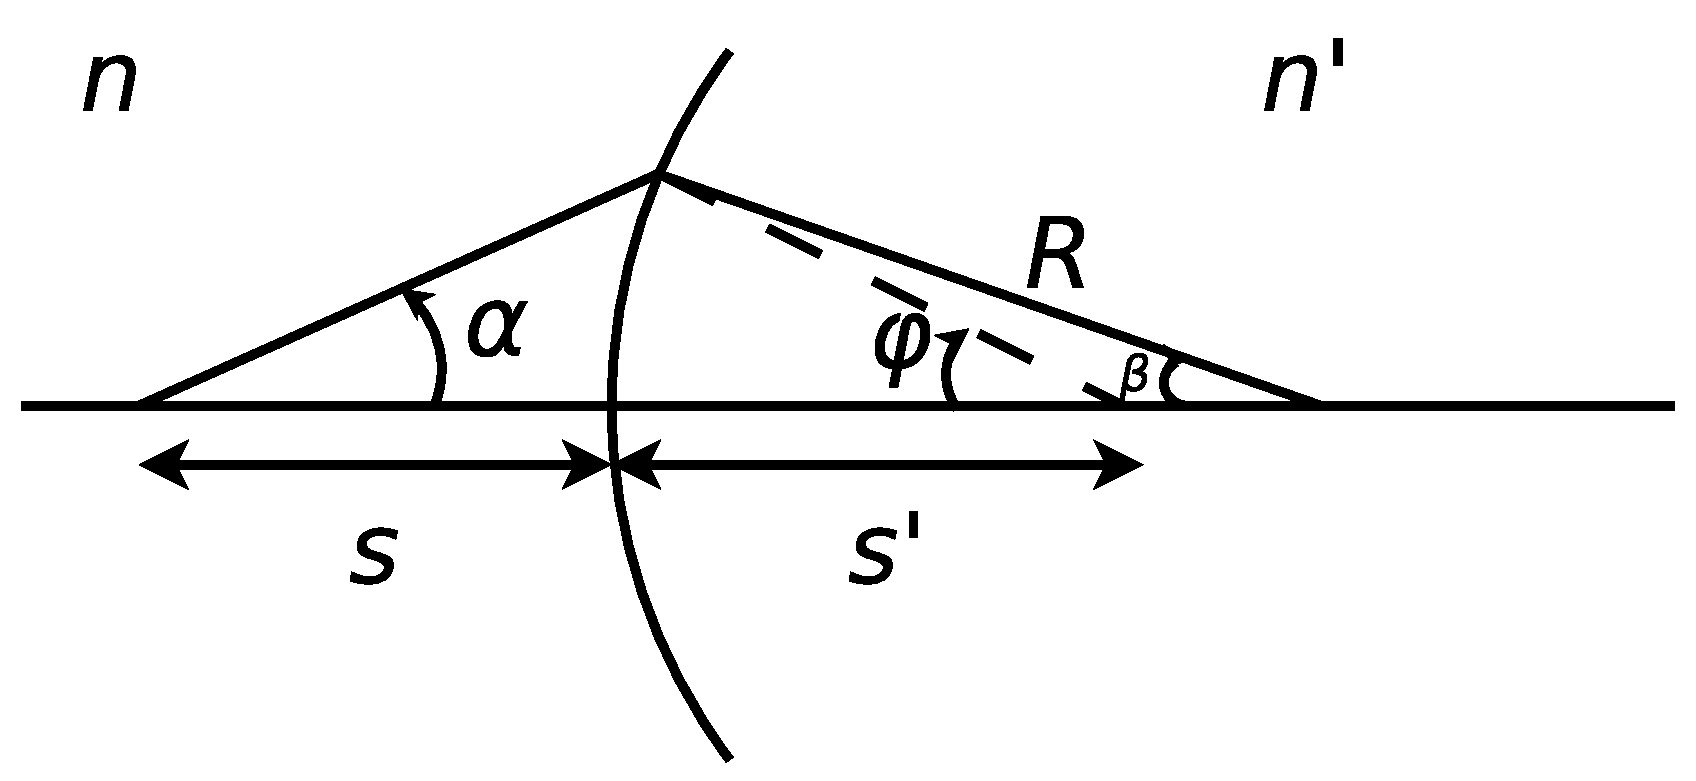
\includegraphics[clip,scale=0.25]{ej3-15}
\end{figure}
\begin{enumerate}
\item Haciendo uso de la figura, de la ley de Snell y del hecho de que en
la aproximación paraxial $\alpha\approx\sin\alpha\approx\tan\alpha$
(lo mismo pasa con $\beta$ y $\varphi$) obtenga la ecuación de las
dioptras esféricas, que establece lo siguiente:
\[
\frac{n'}{s'}\mp\frac{n}{s}=\frac{(n'-n)}{R}
\]
Discuta el doble signo, asociándolo con la convención de signos que
se utilice.
\item Para una dioptra esférica arbitraria haga un gráfico $s'$ vs $s$
y analice a partir de él para qué posiciones de los objetos reales
las imágenes son reales o virtuales, directas o invertidas y lo mismo
para objetos virtuales. Analice todos los casos posibles para dioptras
convergentes y divergentes.
\item ¿Pueden ser iguales las dos distancias focales de una dioptra?. Justifique
su respuesta.
\end{enumerate}


\section*{Doble dioptra}
\item Una barra de material plástico transparente de la forma y dimensiones
de la figura, es iluminada por una rendija. Calcular la posición y
tamaño de la imagen formada por cada una de las dioptras, y especificar
si son reales o virtuales. El índice de refracción es $1.56$. Hacer
un trazado de rayos a escala.
\begin{figure}[H]
\centering{}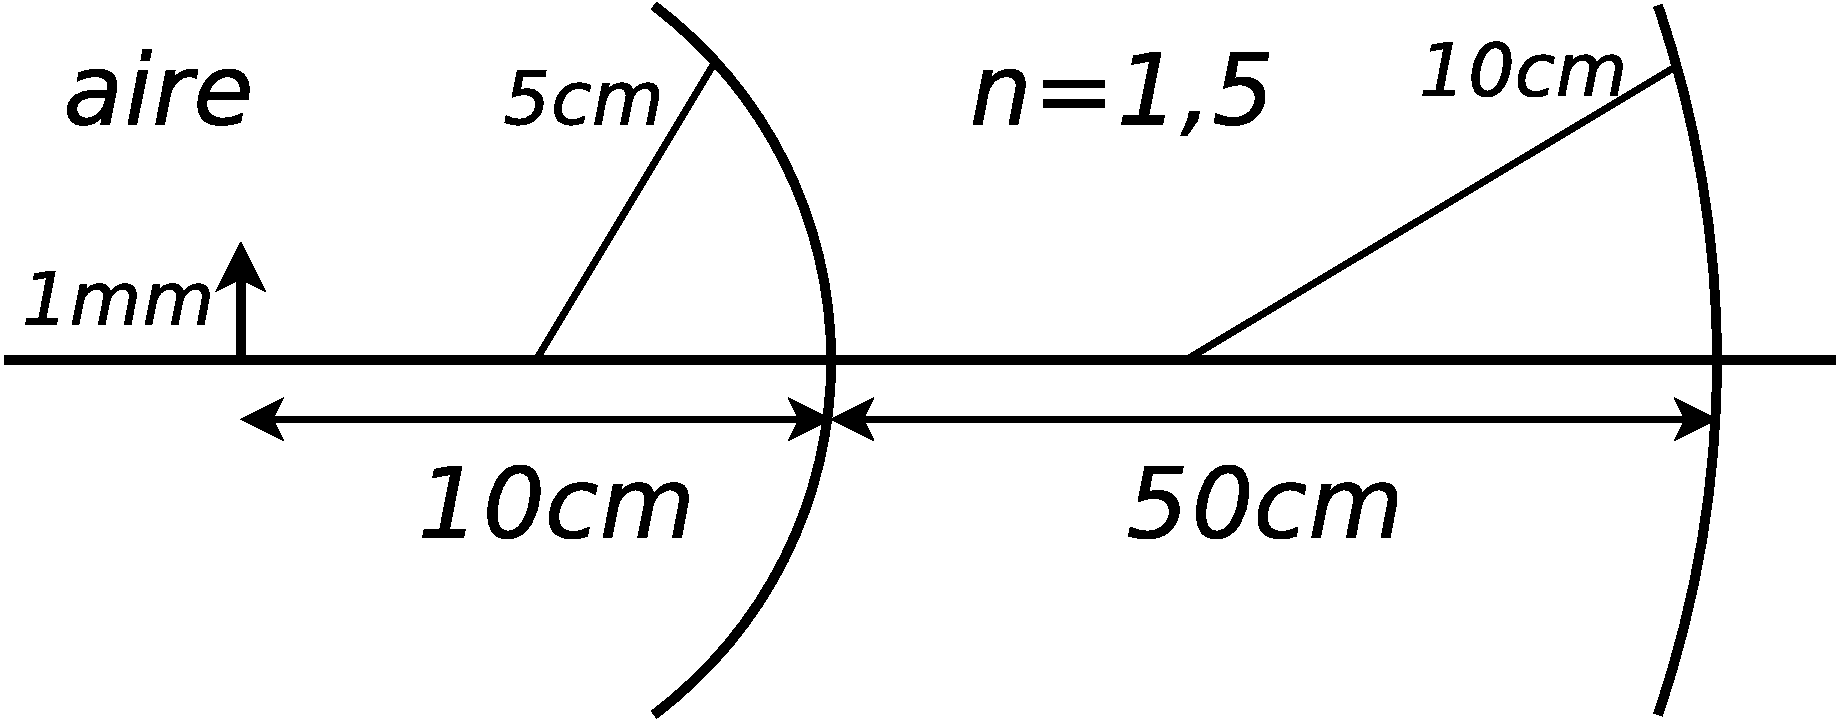
\includegraphics[clip,scale=0.25]{ej3-16}
\end{figure}


\item La esfera de vidrio de la figura, de 1cm de diámetro, contiene una
pequeña burbuja de aire desplazada $0.5$ cm de su centro. Hallar
la posición y el aumento de la burbuja cuando se la observa desde
\emph{A} y cuando se la observa desde \emph{B}.
\begin{figure}[H]
\centering{}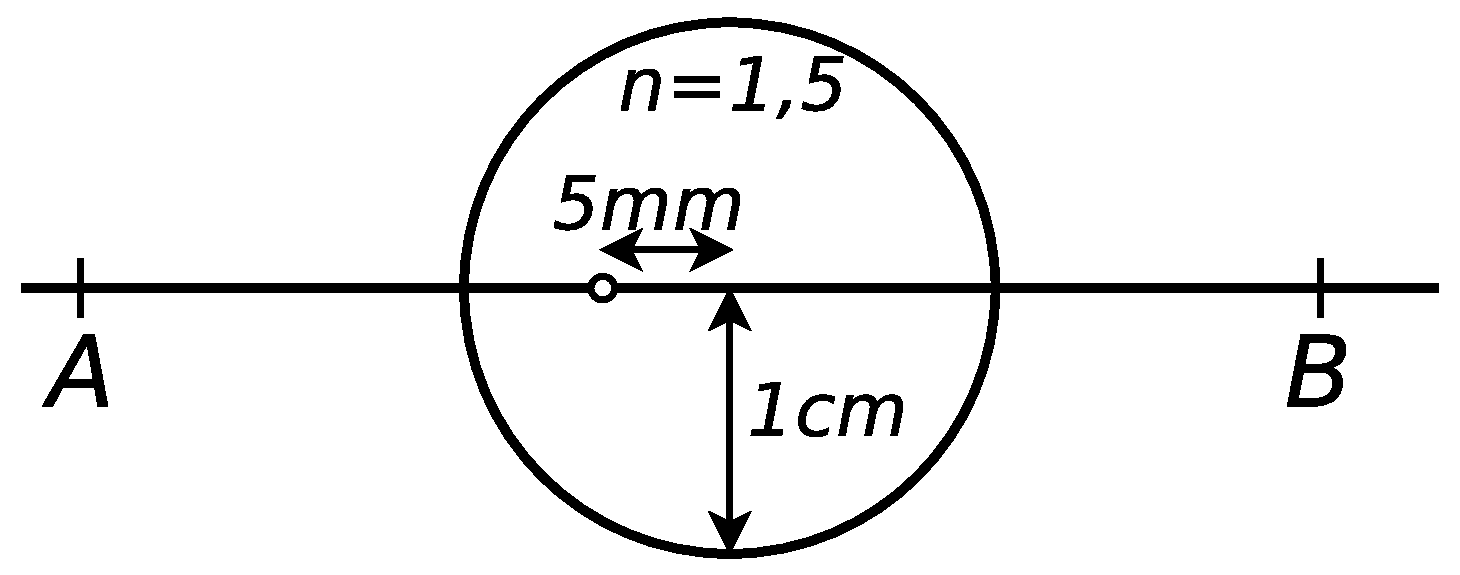
\includegraphics[clip,scale=0.25]{ej3-17}
\end{figure}


\item
\begin{enumerate}
\item Partiendo de la ecuación de las dioptras obtenga la ecuación de los
espejos esféricos. 
\item ¿Cómo se modifica la distancia focal de un espejo esférico si se lo
sumerge en agua?
\item Un espejo esférico cóncavo produce una imagen cuyo tamaño es el doble
del tamaño del objeto, siendo la distancia objeto--imagen de 15 cm.
Calcule la distancia focal del espejo.
\end{enumerate}


\item Una esfera maciza de radio $R$ e índice de refracción $1.5$ ha sido
espejada en una mitad de su superficie. Se coloca un objeto sobre
el eje de la esfera a distancia $2R$ del vértice de la semiesfera
no espejada. Hallar:
\begin{enumerate}
\item La imagen final, en forma analítica, luego de todas las refracciones
y reflexiones que hayan tenido lugar.
\item El aumento y las características de la imagen final.
\item Ídem (a) mediante trazado de rayos.
\end{enumerate}


\section*{Lente delgada}

\item 
\begin{enumerate}
\item A partir de la ecuación de la dioptra, considerando dos dioptras esféricas
tal que la separación entre ellas sea mucho menor que las restantes
longitudes involucradas, deduzca la ecuación para las lentes delgadas.
\item Analice de qué depende la convergencia o divergencia de una lente.
\item Grafique $s'$ vs $s$ para lentes convergentes y divergentes, analice
el aumento y la posición de los objetos (en particular objeto en el
foco y objeto en infinito) y de las imágenes.
\item ¿Pueden ser iguales (en módulo) los focos de una lente?
\item Demuestre que la menor distancia objeto--imagen es $4f$, si la lente
está inmersa en un único medio.
\item Dibuje los frentes de onda incidente, refractado por la primer dioptra
y refractado por la segunda.
\end{enumerate}

% \item ~

\begin{enumerate}
\item Determine la distancia focal de una lente plano--cóncava ($n=1,5$)
cuyo radio de curvatura es 10 cm. Determine su potencia en dioptrías.
\item Se tiene una lente biconvexa con $R_{1}=R_{2}=$10 cm, construida
con un vidrio de índice $1.5$. Se la usa con aire a un lado de la
misma y con un líquido de índice $1.7$ al otro lado. ¿Cuánto valen
las distancias focales? ¿Es convergente o divergente? Responda las
mismas preguntas si: i) está inmersa sólo en aire, ii) está inmersa
en el medio de índice $1.7$.
\end{enumerate}


\item A simple vista la luna subtiende un ángulo de 31'08''. ¿Cuál es el
tamaño de la imagen de la luna, a través de una lente convergente
de distancia focal 1 m?

\item
\begin{enumerate}
\item Se coloca un objeto a 18 cm de una pantalla, ¿en qué puntos entre
la pantalla y el objeto se puede colocar una lente delgada convergente
de distancia focal 4 cm, para que la imagen del objeto esté sobre
la pantalla? ¿Qué diferencia hay entre ubicarla en una u otra posición?
\item Un objeto se halla a distancia fija de la pantalla. Una lente delgada
convergente, de distancia focal 16 cm, produce imagen nítida sobre
la pantalla cuando se encuentra en dos posiciones que distan entre
sí 60 cm. ¿Cuál es la distancia objeto--pantalla?
\end{enumerate}


\item Halle la distancia focal de una lente sumergida en agua, sabiendo
que su distancia focal en el aire es de 20 cm. El índice de refracción
del vidrio de la lente es $1.6$. 


\item Se tiene una lente delgada en las condiciones que presenta la figura.
Indique en qué punto del eje óptico debe incidir un rayo para que
atraviese la lente sin desviarse. Exprese el resultado en función
de la distancia focal objeto y de los índices de refracción.
\begin{figure}[H]
\centering{}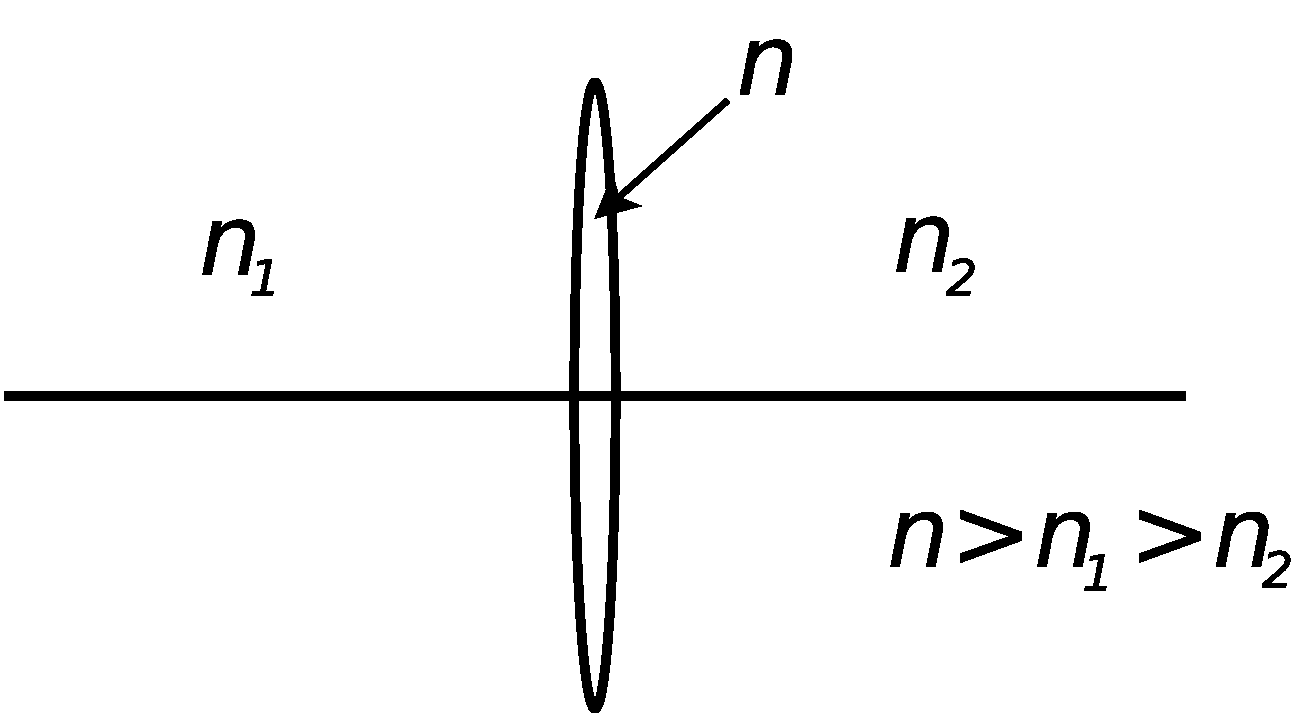
\includegraphics[clip,scale=0.25]{ej3-25}
\end{figure}



\item Demostrar que:
\begin{enumerate}
\item Si un sistema óptico forma imágenes geométricamente perfectas, todos
los rayos que conectan puntos conjugados recorren el mismo camino
óptico. (Utilice el principio de Fermat).
\item Si una lente delgada forma imágenes perfectas sólo en la aproximación
paraxial, la diferencia de caminos ópticos entre dos rayos cualesquiera
que conectan puntos conjugados y que en todo punto disten menos que
$y$, es de orden superior a $y^{2}$.
\end{enumerate}


\item
\begin{enumerate}
\item Determine el radio de curvatura de una lupa equiconvexa ($n=1,5$)
para que su aumento sea 10X. ¿Dónde se encuentra la imagen, y el objeto?
\item Calcule el aumento de la lupa descripta en (a) cuando la imagen se
encuentra a la distancia de visión clara. Discuta las ventajas y desventajas
de esta opción.
\end{enumerate}


\section*{Dos lentes}

\item Una lente delgada convergente, de distancia focal 30 cm, se coloca
20 cm a la izquierda de otra lente delgada divergente de distancia
focal 50 cm. Para un objeto colocado a 40 cm a la izquierda de la
primera lente determine la imagen final. ¿Cuál es el aumento? La imagen
¿es real o virtual, es directa o invertida?


\item Una lente delgada convergente de 5 cm de diámetro y 4 cm de distancia
focal se halla 2 cm a la derecha de un diafragma de 3 cm de diámetro.
\begin{enumerate}
\item Si se coloca un objeto puntual axial a 9 cm a la izquierda de la lente,
determinar la posición y el tamaño de las pupilas de entrada y salida,
en forma gráfica y analítica.
\item Se desplaza al objeto, perpendicularmente al eje óptico, una distancia
de $1.5$ cm. Determine en forma gráfica y analítica, si el diafragma
de apertura está bien definido.
\item Repita el cálculo hecho en (b), cuando el objeto es desplazado una
distancia de 3 cm. Discuta si hay o no vigneteo, y en caso de haberlo
calcule la máxima altura del objeto para que el diafragma de apertura
esté bien definido.
\end{enumerate}



\section*{Dispositivos}
\item Un microscopio consta de un objetivo de 4 mm de distancia focal y
de un ocular de 30 mm de distancia focal. La distancia entre el foco
imagen del objetivo y el foco objeto del ocular es $g=$18 cm. Calcule:
\begin{enumerate}
\item El aumento normal del microscopio.
\item La distancia objeto--objetivo.
\item Sabiendo que el microscopio no cuenta con diafragmas adicionales,
y que la pupila de salida debe ser real, y del mismo diámetro aproximado
que la pupila del ojo ($\approx$12 mm), discuta cuál de las dos lentes
debe ser el diafragma de apertura, cuál debe ser su diámetro y en
qué posición se halla la pupila de salida.
\item Discuta en qué posiciones colocaría un diafragma de campo, y si esta
introducción modifica o no la determinación del diafragma de apertura.
Justifique claramente sus respuestas.
\end{enumerate}


\item Un anteojo astronómico utiliza como objetivo una lente convergente
de 2 m de distancia focal y 10 cm de diámetro, y como ocular una lente
convergente de 4 cm de distancia focal. Determine:
\begin{enumerate}
\item El aumento eficaz.
\item Las características de la primer imagen de la luna y de la imagen
final a través del telescopio. La luna subtiende, a ojo desnudo, un
ángulo de 31'.
\item El largo total del tubo.
\item El mínimo diámetro del ocular para que el objetivo sea diafragma de
apertura. (Recordar que la luna no es puntual, y por ende hay puntos
objeto extra-axiales).
\item Suponiendo que el diámetro del ocular sea de 4 cm, la posición y el
tamaño de la pupila de salida.
\item La posición en que debe colocarse el ojo.
\item La posición en que debe colocarse, de ser posible, un diafragma de
campo.
\item El mínimo diámetro del posible diafragma de campo para que la imagen
de la luna se vea completa.
\end{enumerate}


\item Delante del objetivo de un telescopio y a distancia $s>f'_{ob}$ se
coloca un objeto de altura $h$.
\begin{enumerate}
\item Obtenga la posición de la imagen en función de $f'_{ob}$, $f'_{oc}$
y $s$. 
\item Calcule el tamaño de la imagen y demuestre gráfica y analíticamente
que el aumento lateral es independiente de la posición del objeto.
\end{enumerate}


\item Una cámara fotográfica estándar tiene como objetivo una lente convergente
de 50 mm ($f'$) y usa película de 35$\times$124 mm.
\begin{enumerate}
\item Si se quiere fotografiar objetos que disten del objetivo entre 1 m
e infinito, ¿qué longitud debe tener la rosca que lo mueve?
\item El sistema se halla enfocando sobre la película a un objeto distante
1 m. Analice qué ocurre con la profundidad de campo para objetos distantes
del primero 20 cm. Repita el análisis si el objeto enfocado inicialmente
se hallase a 3 m y a 10 m.
\item Discuta qué sucedería con la longitud de rosca, la profundidad de
campo y la aproximación paraxial si se quisiera fotografiar objetos
distantes 50 cm.
\item Teniendo en cuenta que la película es el diafragma de campo, discuta
los posibles ángulos de campo máximos, calcule los ángulos de campo
asociados a los lados de la película, para un objeto que se encuentra
en el infinito. ¿Cómo varían los ángulos de campo con la posición
del objeto?, ¿cuánto es posible desplazar el objeto para que la variación
no supere el 5\%?
\item Si se quiere fotografiar un árbol de 5 m de altura, y se lo quiere
fotografiar entero, ¿cuál es la mínima distancia a la que hay que
ponerse?
\item Sabiendo que las aperturas inversas de la cámara ($f/D$) varían ente
$1.4$ y 22; calcule los tamaños máximo y mínimo del diafragma. Discuta
cualitativamente el porqué y cómo de las variaciones de tamaño del
diafragma (su relación con la velocidad del objeto, con la de obturación,
con la luminosidad ambiente, etc.)\end{enumerate}
\end{enumerate}


\end{document}
